\documentclass{ctexart}

\usepackage{graphicx} % 插入图片需要引入该宏包
\graphicspath{{assets/},{img/}} % 图片在当前目录下的assets目录,可以添加多个路径

\begin{document}
	\LaTeX 中的插图 \\
	% 语法:\includegraphics[<选项>]{<文件名>}
	% 格式:EPS,PDF,PNG,JPEG,BMP
	
\includegraphics{latex-project-logo} % 文件后缀名,可以加也可以不加。似乎对PNG格式的支持不太好。
	\\
	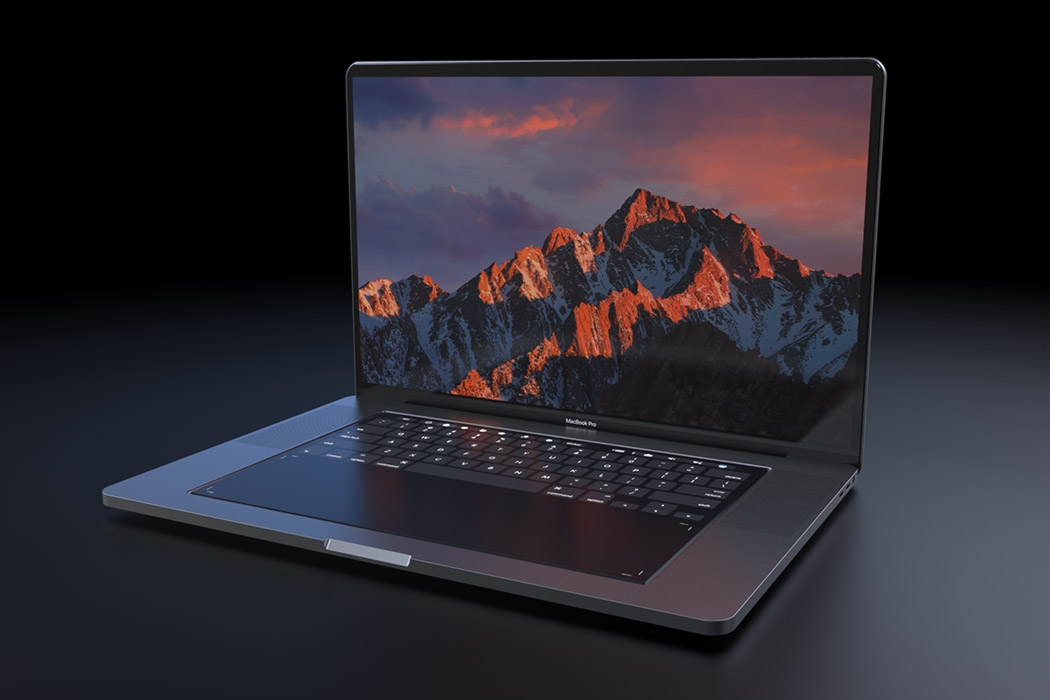
\includegraphics{macbook-1.jpg} % 插图太大,无法正常排版
	\\
	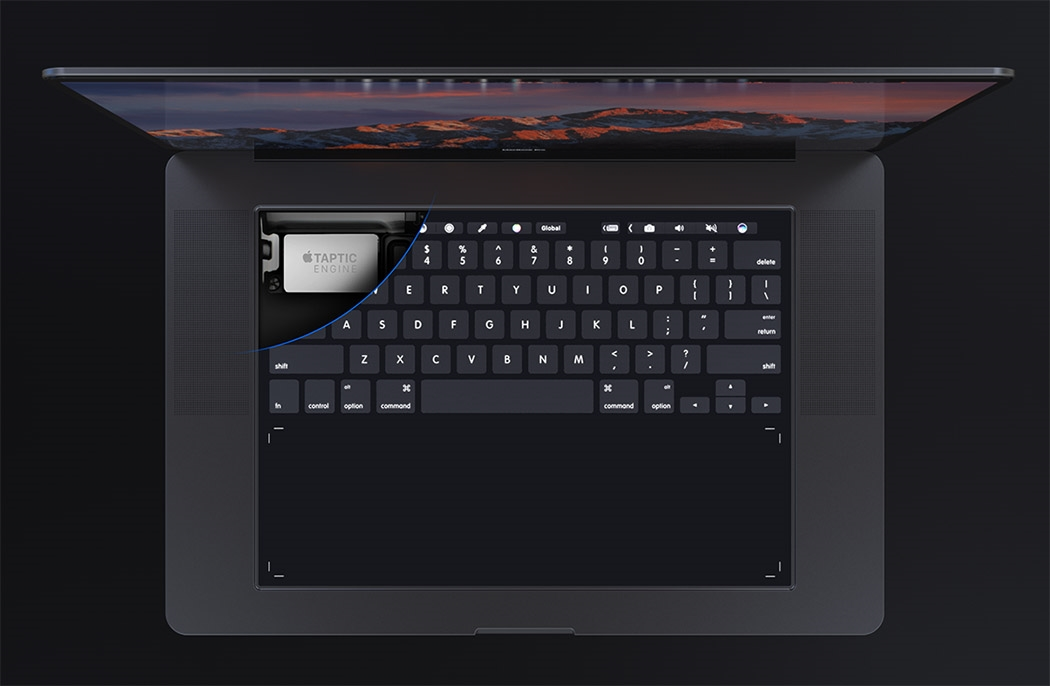
\includegraphics[scale=0.2]{macbook-2.jpg} % 原始比例的0.3倍
	\\
	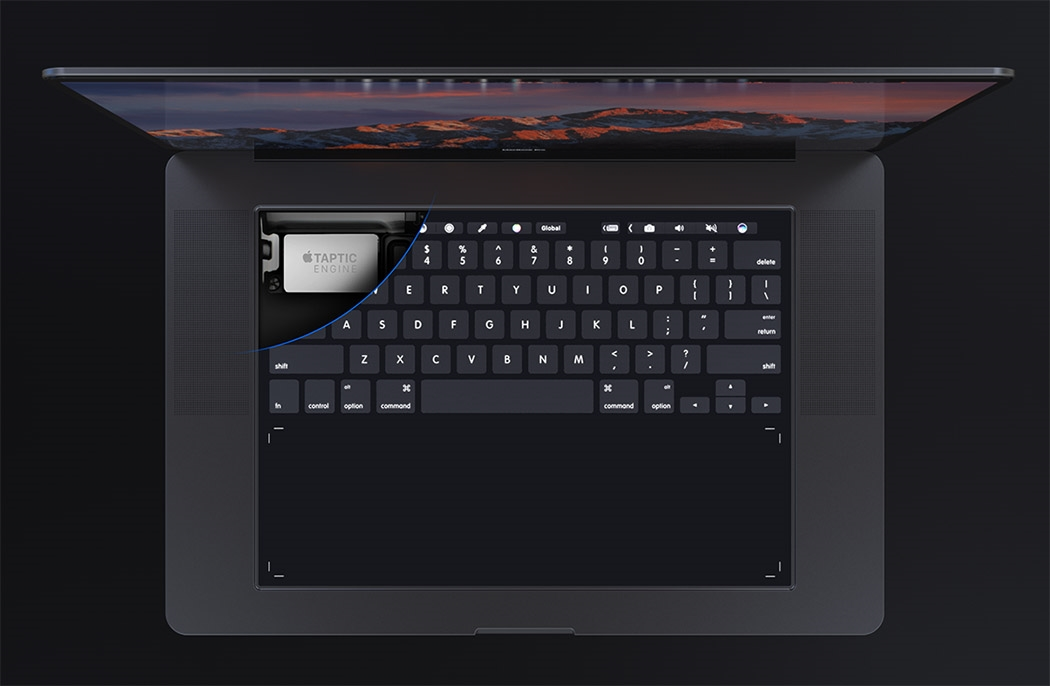
\includegraphics[height=0.2\textheight]{macbook-2.jpg} % 版型高度0.2倍的图像高度
	\\
	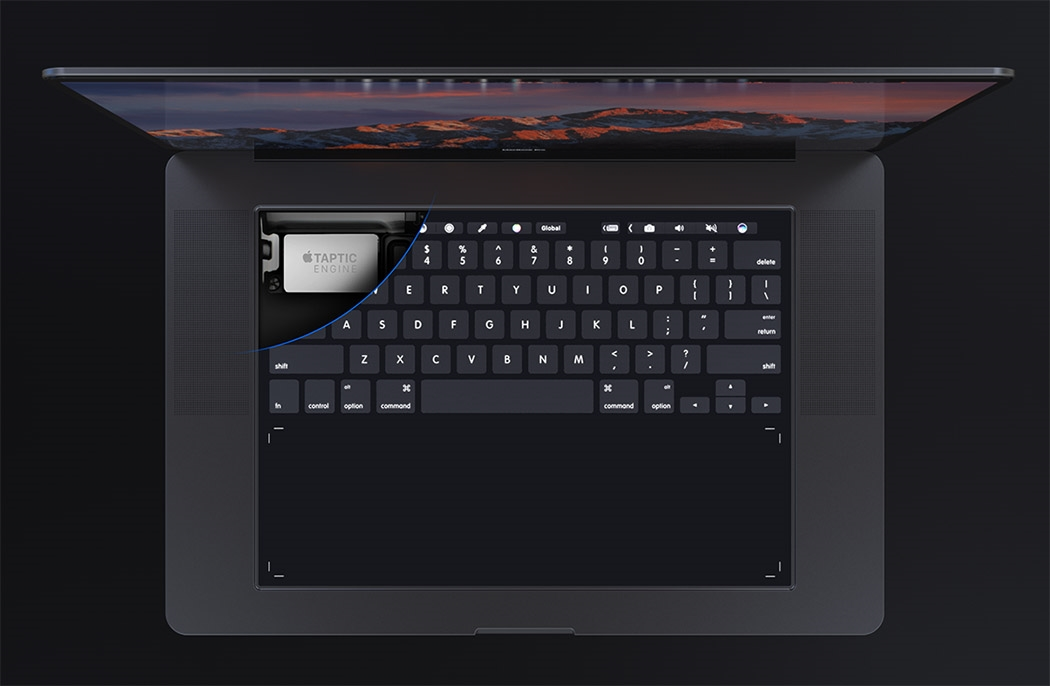
\includegraphics[width=0.2\textwidth]{macbook-2.jpg} % 版型宽度0.2倍的图像宽度
	\\
	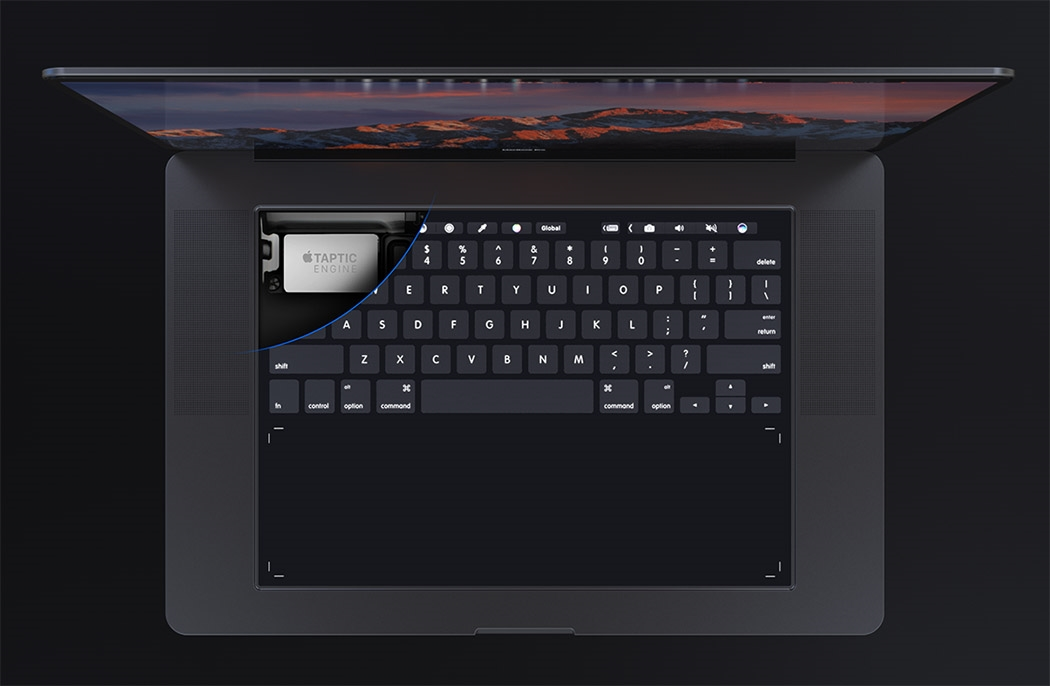
\includegraphics[angle=45, width=0.2\textwidth]{macbook-2.jpg} % 可以使用多个参数
\end{document}